\documentclass[12pt]{article}
\usepackage{amsmath}
\usepackage{graphicx}
\usepackage{hyperref}
\usepackage{listings}
\usepackage{color}
\usepackage{pythonhighlight}

\title{Operating System Course Report - First Half of the Semester}
\author{A class}
\date{\today}

\begin{document}

\maketitle
\newpage

\tableofcontents
\newpage

\section{Introduction}
This report summarizes the topics covered during the first half of the Operating System course. It includes theoretical concepts, practical implementations, and assignments. The course focuses on the fundamentals of operating systems, including system architecture, process management, CPU scheduling, and deadlock handling.

\section{Course Overview}
\subsection{Objectives}
The main objectives of this course are:
\begin{itemize}
    \item To understand the basic components and architecture of a computer system.
    \item To learn process management, scheduling, and inter-process communication.
    \item To explore file systems, input/output management, and virtualization.
    \item To study the prevention and handling of deadlocks in operating systems.
\end{itemize}

\subsection{Course Structure}
The course is divided into two halves. This report focuses on the first half, which covers:
\begin{itemize}
    \item Basic Concepts and Components of Computer Systems
    \item System Performance and Metrics
    \item System Architecture of Computer Systems
    \item Process Description and Control
    \item Scheduling Algorithms
    \item Process Creation and Termination
    \item Introduction to Threads
    \item File Systems
    \item Input and Output Management
    \item Deadlock Introduction and Prevention
    \item User Interface Management
    \item Virtualization in Operating Systems
\end{itemize}

\section{Topics Covered}

\subsection{Basic Concepts and Components of Computer Systems}
This section explains the fundamental components that make up a computer system, including the CPU, memory, storage, and input/output devices.

\subsection{System Performance and Metrics}
This section introduces various system performance metrics used to measure the efficiency of a computer system, including throughput, response time, and utilization.

\subsection{System Architecture of Computer Systems}
Describes the architecture of modern computer systems, focusing on the interaction between hardware and the operating system.

\subsection{Process Description and Control}
Processes are a central concept in operating systems. This section covers:
\begin{itemize}
    \item Process states and state transitions
    \item Process control block (PCB)
    \item Context switching
\end{itemize}

\subsection{Scheduling Algorithms}
This section covers:
\begin{itemize}
    \item First-Come, First-Served (FCFS)
    \item Shortest Job Next (SJN)
    \item Round Robin (RR)
\end{itemize}
It explains how these algorithms are used to allocate CPU time to processes.

\subsection{Process Creation and Termination}
Details how processes are created and terminated by the operating system, including:
\begin{itemize}
    \item Process spawning
    \item Process termination conditions
\end{itemize}

\subsection{Introduction to Threads}
This section introduces the concept of threads and their relation to processes, covering:
\begin{itemize}
    \item Single-threaded vs. multi-threaded processes
    \item Benefits of multithreading
\end{itemize}

\begin{figure}[h]
    \centering
    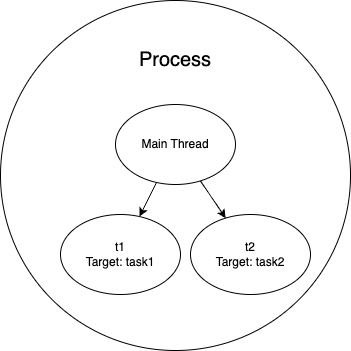
\includegraphics[width=0.5\textwidth]{/Users/khawaritzmi/Unhas/os_report_mid2024/a_class/asset/example.png}  % Sesuaikan nama file dan ukurannya
    \caption{Ini adalah gambar contoh dari multithreading.}
    \label{fig:contoh_gambar}
\end{figure}

Seperti yang terlihat pada Gambar \ref{fig:contoh_gambar}, inilah cara menambahkan gambar dengan keterangan.

\subsection{File Systems}
File systems provide a way for the operating system to store, retrieve, and manage data. This section explains:
\begin{itemize}
    \item File system structure
    \item File access methods
    \item Directory management
\end{itemize}

\setlength{\parindent}{0pt}

\subsection{Input and Output Management}

\setcounter{subsubsection}{3}
\subsubsection{Pengaksesan Input/Output}

\begin{enumerate}
    \item \textbf{Memory Mapped I/O} \\
    Piranti I/O dihubungkan sebagai lokasi memori virtual dimana port I/O tergantung memori utama. \\ 
    Karakteristik:
    \begin{itemize}
        \item Port I/O dihubungkan ke \textit{bus alamat}.
        \item Piranti input sebagai bagian memori yang memberikan data ke \textit{bus data}. Piranti output sebagai bagian memori yang memiliki data yang tersimpan di dalamnya.
        \item Port I/O menempati lokasi tertentu pada ruang alamat dan diakses seolah-olah adalah lokasi memori.
    \end{itemize}
    
    \item \textbf{I/O Mapped I/O (I/O Isolated)} \\
    Piranti I/O dihubungkan sebagai lokasi terpisah dengan lokasi memori, dimana port I/O tidak tergantung pada memori utama. \\
    Karakteristik:
    \begin{itemize}
        \item Port I/O tidak tergantung memori utama.
        \item Transfer informasi dilakukan di bawah kendali sinyal kontrol yang menggunakan instruksi \textit{INPUT} dan \textit{OUTPUT}.
        \item Operasi I/O tergantung sinyal kendali dari CPU.
        \item Instruksi I/O mengaktifkan baris kendali \textit{read/write} pada port I/O, sedangkan instruksi memori akan mengaktifkan baris kendali \textit{read/write} pada memori.
        \item Ruang memori dan ruang alamat I/O menyatu, sehingga dapat memiliki alamat yang sama.
    \end{itemize}
\end{enumerate}

\subsubsection{Skema Komputer}

\begin{figure}[h]
    \centering
    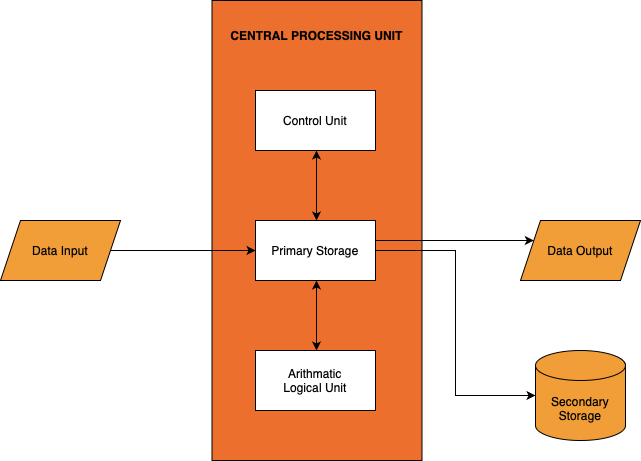
\includegraphics[width=0.6\textwidth]{/asset/skema_komputer.png}
    \caption{Diagram sistem komputer}
\end{figure}

Diagram ini menunjukkan alur data. Proses yang digambarkan dimulai dengan \textit{data input} yang masuk ke dalam sistem dan dikirim ke \textit{Central Processing Unit (CPU)}. Di dalam CPU, \textit{control unit} mengambil instruksi dari \textit{primary storage} (memori utama) dan mengarahkan data tersebut ke \textit{arithmetic logical unit (ALU)} untuk melakukan operasi aritmatika dan logika.\vspace{10pt}

Setelah data diproses, hasilnya dapat disimpan sementara di \textit{primary storage} atau permanen di \textit{secondary storage}, kemudian hasil akhirnya dikeluarkan melalui \textit{data output} untuk digunakan oleh pengguna atau perangkat lain. Proses ini berlangsung berulang-ulang dalam berbagai operasi komputasi.

\subsubsection{Model Mesin Komputer}

\begin{figure}[h]
    \centering
    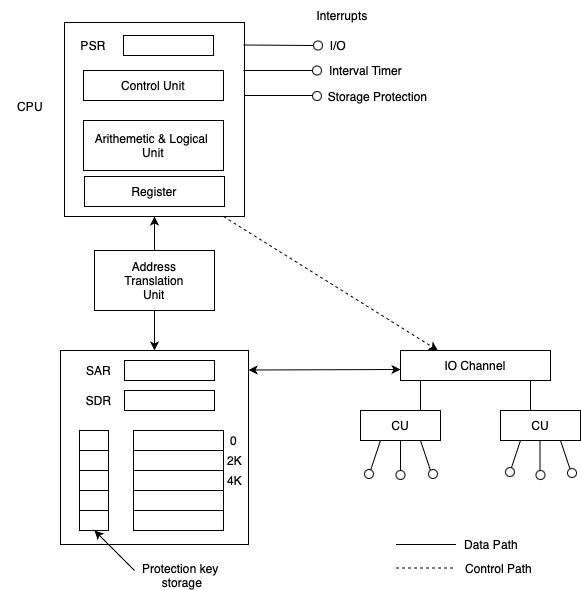
\includegraphics[width=0.6\textwidth]{/asset/model_mesin.png}
    \caption{Diagram model mesin komputer}
\end{figure}

Diagram ini menggambarkan interaksi antara CPU, memori utama, dan saluran \textit{input/output (I/O)} dalam sistem komputer. CPU terdiri dari beberapa komponen utama seperti \textit{Program Status Register (PSR)}, \textit{Control Unit}, \textit{Arithmetic & Logical Unit (ALU)}, dan \textit{Register}.\vspace{10pt}

\textit{Control Unit} mengatur jalannya instruksi dan aliran data, sementara \textit{ALU} menangani operasi aritmatika dan logika. Data dan instruksi dari memori utama diterjemahkan oleh \textit{Address Translation Unit}, yang mengubah alamat logis menjadi alamat fisik. \textit{Main storage} (memori utama) berisi \textit{Storage Address Register (SAR)} dan \textit{Storage Data Register (SDR)} untuk menyimpan alamat dan data yang sedang diakses, serta memiliki \textit{Protection Key Storage} untuk mengatur akses terhadap data dengan kunci proteksi.\vspace{10pt}

Saluran \textit{I/O (I/O Channel)} mengelola komunikasi data antara perangkat \textit{input/output} dan memori, dengan bantuan \textit{Control Unit (CU)} yang terhubung ke perangkat eksternal. CPU dapat menerima interupsi dari perangkat I/O, timer interval, atau proteksi penyimpanan untuk memprioritaskan atau menunda proses tertentu.

\subsection{Deadlock Introduction and Prevention}
Explores the concept of deadlocks and methods for preventing them:
\begin{itemize}
    \item Deadlock conditions
    \item Deadlock prevention techniques
\end{itemize}

\subsection{User Interface Management}
This section discusses the role of the operating system in managing the user interface. Topics covered include:
\begin{itemize}
    \item Graphical User Interface (GUI)
    \item Command-Line Interface (CLI)
    \item Interaction between the user and the operating system
\end{itemize}

\subsection{Virtualization in Operating Systems}
Virtualization allows multiple operating systems to run concurrently on a single physical machine. This section explores:
\begin{itemize}
    \item Concept of virtualization
    \item Hypervisors and their types
    \item Benefits of virtualization in modern computing
\end{itemize}

\section{Assignments and Practical Work}
\subsection{Assignment 1: Process Scheduling}
Students were tasked with implementing various process scheduling algorithms (e.g., FCFS, SJN, and RR) and comparing their performance under different conditions.
\subsubsection{Group 1}
\begin{python}
    class Process:
    def __init__(self, pid, arrival_time, burst_time):
        self.pid = pid
        self.arrival_time = arrival_time
        self.burst_time = burst_time
        self.completion_time = 0
        self.turnaround_time = 0
        self.waiting_time = 0
\end{python}

\begin{table}[htbp] % Optional: For floating position
    \centering
    \begin{tabular}{|c|c|c|} % Defines number of columns and alignment (c = center, l = left, r = right). '|' creates vertical lines.
    \hline
    Header 1 & Header 2 & Header 3 \\ % Column headers
    \hline
    Row 1, Column 1 & Row 1, Column 2 & Row 1, Column 3 \\ % First row of data
    \hline
    Row 2, Column 1 & Row 2, Column 2 & Row 2, Column 3 \\ % Second row of data
    \hline
    \end{tabular}
    \caption{Your table caption} % Optional: For adding a caption
    \label{tab:your_label} % Optional: For cross-referencing the table
\end{table}
\subsection{Assignment 2: Deadlock Handling}
In this assignment, students were asked to simulate different deadlock scenarios and explore various prevention methods.
\subsubsection{Group 9}

In this task, we simulate a potential deadlock scenario and implement a deadlock prevention strategy. Two processes, Process 1 and Process 2, each require two resources: Resource A and Resource B.

\subsection*{Deadlock Simulation}

In the deadlock simulation, Process 1 first locks Resource A and waits for Resource B, while Process 2 locks Resource B and waits for Resource A. This creates a circular wait condition, which leads to a deadlock.

\subsection*{Deadlock Prevention}

To prevent the deadlock, we apply a consistent resource allocation order. Both processes are required to lock Resource A first, followed by Resource B. This ensures that no circular wait occurs, and thus avoids the deadlock.\vspace{10pt}

	\lstset{ 
		language=Python,
		backgroundcolor=\color{white}, 
		commentstyle=\color{gray}, 
		keywordstyle=\color{blue},
		basicstyle=\ttfamily\footnotesize, 
		breaklines=true,  
		frame=single, 
		showstringspaces=false, 
	}

\begin{lstlisting}
import threading
import time

# Create two locks to represent Resource A and Resource B
resource_a = threading.Lock()
resource_b = threading.Lock()

# Function for Process 1
def process_1():
    print("Process 1: Requesting Resource A...")
    resource_a.acquire()
    print("Process 1: Acquired Resource A.")
    
    time.sleep(1)  # Simulating work with Resource A
    
    print("Process 1: Requesting Resource B...")
    resource_b.acquire()
    print("Process 1: Acquired Resource B.")
    
    # Release resources after processing
    resource_b.release()
    resource_a.release()
    
    print("Process 1: Released both resources.")

# Function for Process 2
def process_2():
    print("Process 2: Requesting Resource B...")
    resource_b.acquire()
    print("Process 2: Acquired Resource B.")
    
    time.sleep(1)  # Simulating work with Resource B
    
    print("Process 2: Requesting Resource A...")
    resource_a.acquire()
    print("Process 2: Acquired Resource A.")
    
    # Release resources after processing
    resource_a.release()
    resource_b.release()
    
    print("Process 2: Released both resources.")

# Simulating Deadlock
print("Starting simulation of potential deadlock...")

# Create two threads for Process 1 and Process 2
t1 = threading.Thread(target=process_1)
t2 = threading.Thread(target=process_2)

# Start the threads
t1.start()
t2.start()

# Join threads back to the main thread to finish execution
t1.join()
t2.join()

print("Simulation of potential deadlock complete.\n")

# Deadlock Prevention using a consistent resource allocation order
print("Starting deadlock prevention simulation...")

def process_1_prevent_deadlock():
    print("Process 1 (Prevent): Requesting Resource A...")
    resource_a.acquire()
    print("Process 1 (Prevent): Acquired Resource A.")
    
    time.sleep(1)  # Simulating work with Resource A
    
    print("Process 1 (Prevent): Requesting Resource B...")
    resource_b.acquire()
    print("Process 1 (Prevent): Acquired Resource B.")
    
    # Release resources after processing
    resource_b.release()
    resource_a.release()
    
    print("Process 1 (Prevent): Released both resources.")

def process_2_prevent_deadlock():
    print("Process 2 (Prevent): Requesting Resource A...")
    resource_a.acquire()
    print("Process 2 (Prevent): Acquired Resource A.")
    
    time.sleep(1)  # Simulating work with Resource A
    
    print("Process 2 (Prevent): Requesting Resource B...")
    resource_b.acquire()
    print("Process 2 (Prevent): Acquired Resource B.")
    
    # Release resources after processing
    resource_b.release()
    resource_a.release()
    
    print("Process 2 (Prevent): Released both resources.")

# Using consistent resource allocation order (A -> B) to prevent deadlock
t1_prevent = threading.Thread(target=process_1_prevent_deadlock)
t2_prevent = threading.Thread(target=process_2_prevent_deadlock)

# Start the threads
t1_prevent.start()
t2_prevent.start()

# Join threads back to the main thread to finish execution
t1_prevent.join()
t2_prevent.join()

print("Deadlock prevention simulation complete.")
\end{lstlisting}

\subsection*{Explanation}
\begin{itemize}
    \item \textbf{Deadlock Simulation}: In this part, we simulate a deadlock where Process 1 locks Resource A and waits for Resource B, while Process 2 locks Resource B and waits for Resource A. This leads to a circular wait (deadlock).
    \item \textbf{Deadlock Prevention}: In the second part, we use a consistent resource allocation order, where both processes request Resource A first and then Resource B. This prevents deadlock because no circular wait can occur.
\end{itemize}

\subsection{Assignment 3: Multithreading and Amdahl's Law}
This assignment involved designing a multithreading scenario to solve a computationally intensive problem. Students then applied **Amdahl's Law** to calculate the theoretical speedup of the program as the number of threads increased.

\subsection{Assignment 4: Simple Command-Line Interface (CLI) for User Interface Management}
Students were tasked with creating a simple **CLI** for user interface management. The CLI should support basic commands such as file manipulation (creating, listing, and deleting files), process management, and system status reporting.

\subsection{Assignment 5: File System Access}
In this assignment, students implemented file system access routines, including:
\begin{itemize}
    \item File creation and deletion
    \item Reading from and writing to files
    \item Navigating directories and managing file permissions
\end{itemize}

\section{Conclusion}
The first half of the course introduced core operating system concepts, including process management, scheduling, multithreading, and file system access. These topics provided a foundation for more advanced topics to be covered in the second half of the course.

\end{document}